% %This is a very basic article template.
% %There is just one section and two subsections.
\documentclass[authoryear, review,12pt,number]{elsarticle}
\usepackage[numbers]{natbib}
%\usepackage{citep}
\usepackage{graphicx}
\usepackage{float}
\usepackage{rotating}
\usepackage{stfloats}
\usepackage{lineno}
\usepackage[linesnumbered,ruled,vlined]{algorithm2e}
\usepackage{tabulary}
\usepackage{graphicx}
\usepackage{color}
\usepackage[none]{hyphenat}
\usepackage[table]{xcolor}
\sloppy
\begin{document}

\begin{frontmatter}
\linenumbers
\title{Automated Classifying of EUNIS Habitats with Ontologies and Data Mining
methods}


\author[TUB]{T. Niklas Moran\corref{cor1}}
\ead{niklasmoran@mailbox.tu-berlin.de}

\author[TUB]{Simon Nieland}
\author[TUB]{Birgit Kleinschmit}

%\author[TUB]{Michael F\"orster}

\address[TUB]{Geoinformation in Environmental Planning Lab, Technische
Universit\"at Berlin, Stra\ss e des 17. Juni 145, 10623 Berlin, Germany}

\cortext[cor1]{Corresponding author at: Geoinformation in Environmental Planning
Lab, Technische Universit\"at Berlin, Stra\ss e des 17. Juni 145, 10623 Berlin,
Germany}  % el.:+49 30 314 72601;}

\begin{abstract}
Write some text here..
\end{abstract}

\begin{keyword}
remote sensing, biotope classification, data mining,
generalisation, nature conservation, OWL2, EUNIS, OBIA
\end{keyword}

\end{frontmatter}

\linenumbers

\section{Introduction} 
% NATURA2000 obligations and local obligations = NATFLO
Recognizing that human-caused habitat destruction plays a dominant role in
biodiversity loss, the European Union has implemented an environmental
conservation framework to halt biodiversity loss in accordance with the
Convention on Biological Diversity (CBD, 2005). An integral part of this
framework is the EU Habitats Directive (Council Directive) 92/43/EEC [1992],
which established the Natura 2000 network of habitats. The law requires
conservation and monitoring of designated habitats by member states and for a
report to be submitted every six years. Environmental data 
to determine biodiversity status must be collected to comply with the 
statute. Comparing environmental data used for these reports can be 
difficult due to varying data collection methods by the 
nature conservation authorities in each member state. Therefore, technical 
solutions to increase interoperability by thematically harmonizing 
environmental data is needed. International policy-making would benefit from 
thematic harmonization and could better assess and compare outcomes. Due to 
these obligations and other environmental and spatial planning requirements, 
the German federal state of
Rhineland-Palatinate (RLP) created the NATFLO project (Landscape objects from
remotely sensed data for nature conservancy).\\
The aim of the NATFLO project is to implement a
thematically integrated state-wide system with all relevant geo-data for plans
and decision-making at all levels of government.  Since collection of
comprehensive, high quality environmental data through field recordings is
expensive and time consuming, the project harnesses existing environmental data
and remote sensing products. To increase semantic interoperability and
automation, vector objects with various indices are used with concepts from the
Eionet Action Group on Land monitoring in Europe (EAGLE) and EU-wide 
biotope classification schema called EUNIS).\\
In this paper we propose an automated system that can classify nature protection
areas according to EUNIS using EO data, an existing biotope map
and expert knowledge formalized in an ontology. The biotope data serves as class
labels for training data mining algorithms which generate rules that can be
imported into an ontology. Once the rules and segmented objects are imported
into an ontology, a reasoner can perform A-box and T-box reasoning classifying
which objects belong to which class and how the classes are related. This method
contributes to the goal of empirically-deriven rule creation and enhances
data interoperability and comparison.
\section{Method}
This section describes the developed method for classifying EUNIS habitats by
using data mining algorithms to generate rules based on digital surface
model (DSM) and digital terrain model (DTM) derived zonal statistics and remote
sensing data of pre-segmented polygons.
Furthermore the method's advantage over a purely data mining approach is
the creation of an ontology in the Web Ontology Language (OWL2/XML) that
increases the interoperablity and readability of results. The benefits of using
ontologies is described below.
\subsection{Formalization of Expert Knowledge}
With the help of an ecologist, RLP biotope classes (OSIRIS) were converted
to the appropriate EUNIS class and indicators were developed for habitat
classification. We use indicators from the classification schemes and concepts
from EAGLE to create a comprehensive interoperable vocabulary. This process
involved attaching indicators from EUNIS, NATFLO and EAGLE to each biotope.
For example, the parameter ``wetness'' could be any of ``dry'', ``mesic",
``wet'' or ``very wet'', but for EUNIS class E1 - dry grasslands would be
``dry''. An example of how the classes were  modeled in Prot\'eg\'e is shown in
figure 1. As one can see in the diagram, E1.72 is a subclass of E1.7 with the
dominant plant species ``Agrostis''.
$$ E1.72 \equiv  E1.7 \sqcap \exists dominant\_plant\_species
\{``Agrostis'' \}$$
$$
dry \equiv rule\_1 \sqcap rule\_2 \sqcap rule\_3
$$
\begin{figure}
	
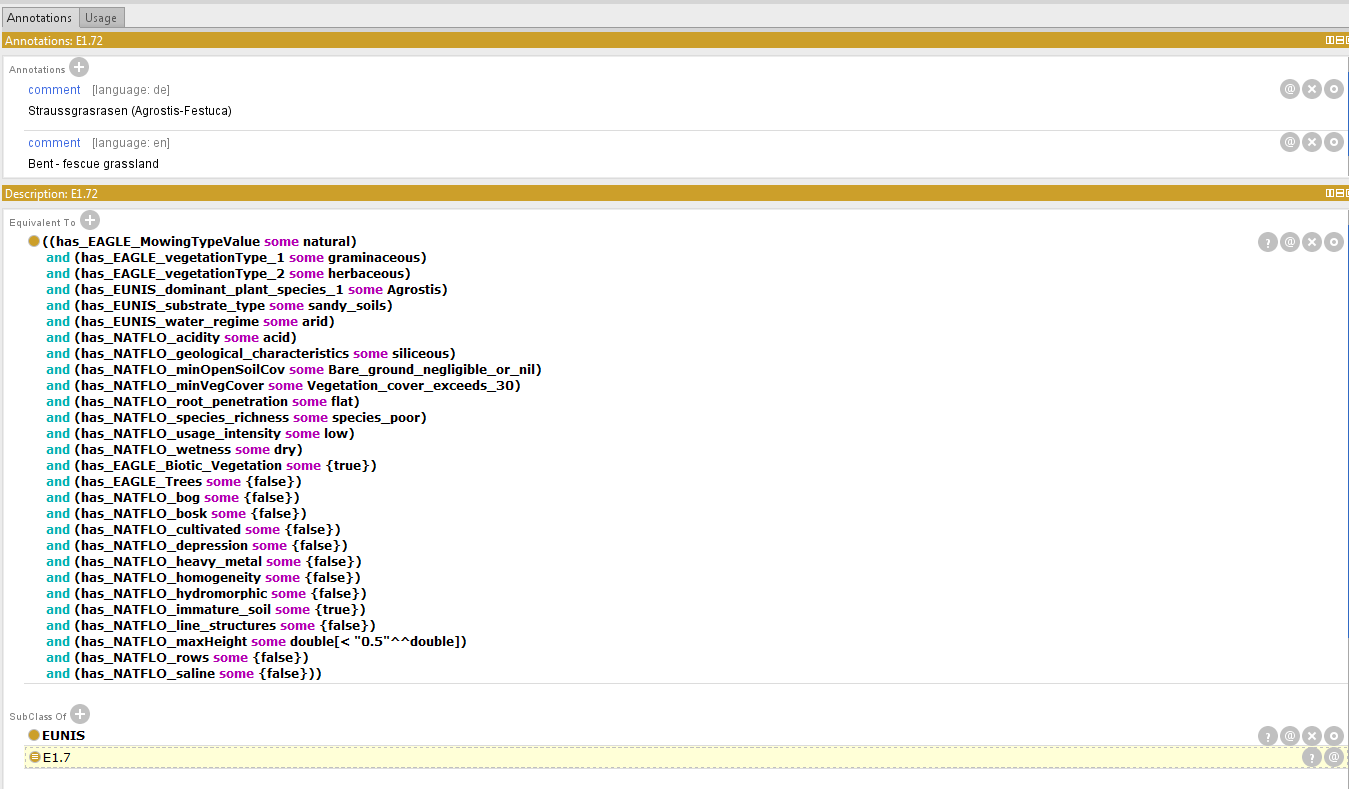
\includegraphics[width=1\linewidth]{diagrams/protege_description_eunis.PNG}
	\caption{Prot\'eg\'e vizualization of the OWL2/XML EUNIS classes present in
	RLP}
\end{figure}


\subsection{Data and Pre-Processing}
All input data comes from the RLP Ordnance Survey (Landesamt f\"ur Vermessung 
und Geobasisinformation). The data is segmented by RLP AgroScience using
multi-spectral (B, G, R, NIR) orthophotos with a 0.2m ground resolution and a
2 x 2km tile size. The orthophotos are updated every 2 years and are used to
create the Digital Surface Model (DSM) using automated stereo matching. The
Digital Terrain Model(DTM) and Digital Elevation Model (DEM) was produced using
LiDAR ASCII point clouds acquired between 2003 and 2009 with a resolution of
0.5m.\\
\subsection{Segmentation}
The iterative object-based image analysis is performed using Defiens eCognition Server
and segments the data using thresholds and multi-resolution approaches (Baatz and
Sch\'ape 2000). The segmentation process uses information solely from aerial
images based on spectral information (NDVI and Bare Area Index) and
height from the digital elevation model (DEM) to separate
between biotic and no-biotic features \citep{Tintrup2015}. 
The detailed pre-processing workflow is shown in figure XX.
%EAGLE nomenclature for landcover classes.
\begin{figure}
	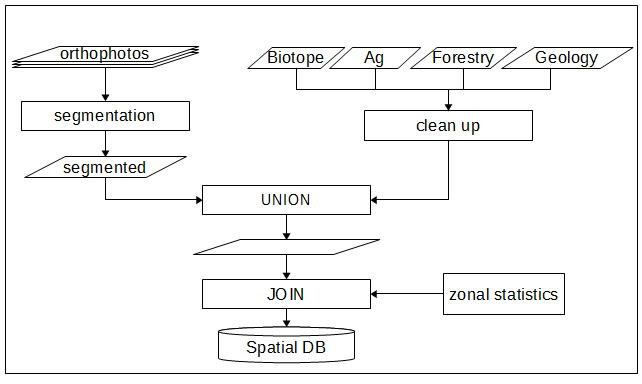
\includegraphics[width=1\textwidth]{diagrams/pre_processing.png}
	\caption{Ag - agriculture map}
\end{figure}

The basic pre-processing steps are outlined below.
\begin{enumerate}
    \item Clip the biotope, agriculture, forestry and geology maps to the extent
    of Saarburg
    \item Join EUNIS properties to OSIRIS class names
    \item Postgis join using ST\_WITHIN to select segmented polygons
    completely within biotope map polygons
    \item Join zonal statistics to the segmented polygons
\end{enumerate}

\begin{figure}
	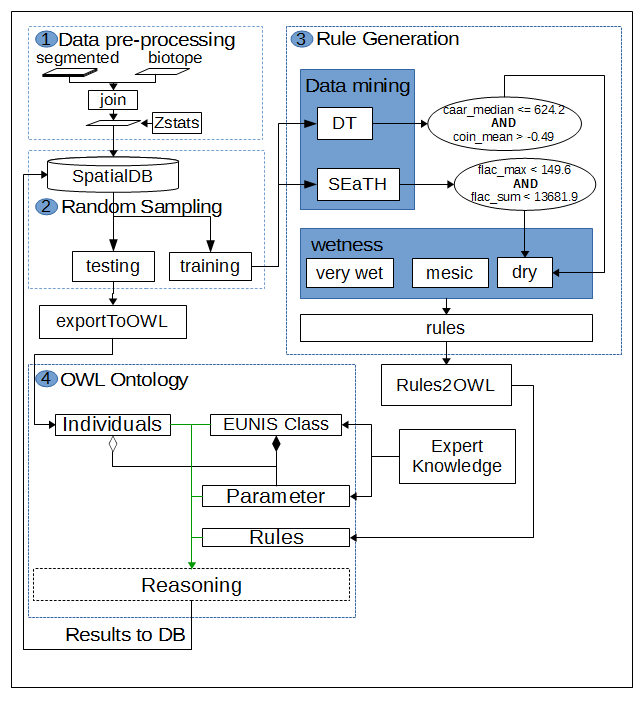
\includegraphics[width=1\linewidth]{diagrams/another_workflow_diagram_large.png}
	\caption{1)Detailed pre-processing is shown in figure 2 and described in the
	text.
	2) Create training and testing tables in the database for use by 3) 
Rules generated by the data mining algorithms are converted into OWL2/XML }
\end{figure}
We apply a PostGIS spatial join query using ST\_WITHIN to select only those
polygons from the segmented dataset that fall completely within the biotope
polygon of our pre-processed biotope map. We join those polygons
with EUNIS characteristics and also attach zonal statistics that are calculated
for every polygon. The last step in the pre-processing workflow is the
replacement of any NULL values with zeros. 
The null values arise due to small polygon sizes created by the segmentation
process. In the future, a new segmented dataset that respects the biotope
boundaries should be available and will reduce the problems from selecting
polygons that fall completely within
% the polygon.
%\begin{figure}
%  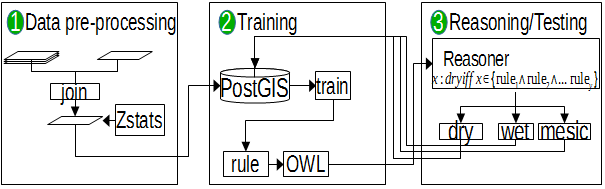
\includegraphics[width=1\linewidth]{diagrams/workflow_overview2.png}
%\caption{A small overview.}
%\end{figure}
The first step was to clip the biotope map with the extent of Saarburg.
Then we join the expert knowledge-derived table that translates the OSIRIS
biotopes to the corresponding EUNIS biotope class. We then perform a spatial
join using PostGIS ST\_WITHIN to select the segmented polygons that lie within
the biotope map. These polygons have all the biotope information
attached to them and in the final step have the zonal statistics with
morphological and hydrological (SAGA wetness index, ) and topographic indices 
(topographic wetness index, ). 
After joining EUNIS characteristics to the RLP
biotope map, the map was spatially joined with the pre-segmented remote sensing
data. software was used for the segmentation and was performed by RLP AgroScience. 
%The remote sensing data already had zonal statistics computed for all of the
%polygons. A list of the zonal statistics are below.
%% INSERT LIST?
\subsection{Rule Generation - Data Mining}
We chose supervised classification algorithms that are able to exploit expert
knowledge, perform classification tasks quickly and accurately and produce human
understandable rule sets for further scrutiny and refinement. Therefore, the
SEaTH algorithm and the Decision Tree algorithm (a type of classification and regression
tree from scikit-learn) were selected to find the optimal combination of 
environmental indices and
object properties that differentiate between objects. The labels used to
differentiate between polygons come from the Rhineland Palatinate biotope map
last updated in 2015. Consulting with experts, the translation between the
Rhineland-Palatinate (OSIRIS) biotopes and EUNIS was possible. The properties of
the EUNIS biotopes was then given to each polygon of the segmented data that
fit within the biotope boundary.
% Nieland, Kleinschmit, F\'orster 2015
\subsection{Selection of Algorithm - SEaTH and Decision Trees}
We first chose the Separability and Thresholds
(SEaTH) \citep{Nussbaum2006} algorithm to automatically derive features important
for classification from the data because it is able to generate rules with
thresholds that can easily be transferred to an ontology. Saving the rules in
the ontology makes it clear what rules were used for classification and can be
used by experts to modify the rules to be more accurate. To compare
classification accuracy we selected the scikit-learn python suite
\citep{scikit-learn} due to its maturity and ease of use and the availability of
different algorithms. We settled on the ``Decision Tree Classifier'' as one can
visualize the results and parse the tree to load the results into the ontology.
Moreover, the automated system can use other algorithms as they become available.
\subsection{SEaTH} The Separability and Thresholds (SEaTH) algorithm
\citep{Nussbaum2006} statistically identifies characteristic features and their thresholds. It has
been used on remote sensing data for land cover classification \citep{Gao2011}
and nuclear installation classification \citep{Nussbaum2006}.
Using training data, the algorithm determines the separability of the object
classes and then calculates the thresholds for which the maximum separability
can be achieved using the given features. One benefit of the algorithm is that
one does not need many training objects.
In the Nussbaum, Niemeyer and Canty (2006) paper, for example, the authors
suggest using only very characteristic features for training and only used
around 10 samples per class\citep{Nussbaum2006}. The authors also state that
usually two features per class is enough to produce accurate results. Combining
this algorithm with an ontology would produces traceable results that are easy
to understand. This approach would also help fill the observation-based ontology
research gap as first described by Janowicz (2012) \citep{Janowicz2012}.

\subsection{Decision Tree Classifier}
The decision tree (DT) classifier implemented in scikit-learn is a modified
classification and regression tree (CART)\citep{scikit-learn}. A cross
validation using DT with many different parameters is first performed to find the best
parameters. Then the rules generated by the algorithm is converted with an
automated python script to OWL Ontology rules.

\subsection{Comparison with Random Forest}
\subsection{Study Area}
%% southwestern?!
Saarburg is an 200km$^{2}$ administrative district part of Trier, located in the
south-west of the federal state of Rhineland Palatinate (RLP), Germany.
Luxembourg borders the area to the west and the federal state of Saarland to the South.
RLP has a western european atlantic climate and has an
economically and culturally important viticulture industry along the Mosel and
Rhine rivers.
\begin{figure}
	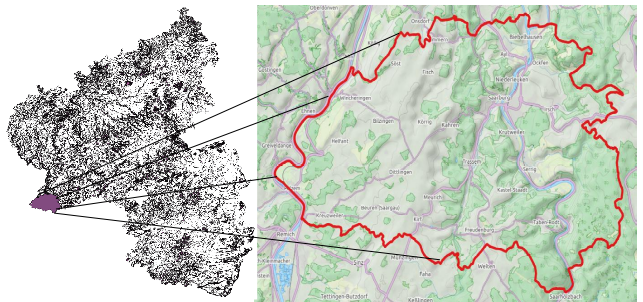
\includegraphics[width=\textwidth]{diagrams/study_area_closeup.png}
	\caption{The location of Saarburg on the left in purple in relation to 
Rheinland Palatinate. The right is from Open Streetmaps Landscape layer. }
\end{figure}

\subsection{Validation}
To create training data, we randomly select 200 training objects per class. A
subset of these objects, 20 per class, are used to train the SEaTH
algorithm as it performs better with fewer characteristic objects. To test the 
results 600 objects per class are selected that are not in the training class.

\section{Results}
This can potentially reduce the amount of features
and statistics that need to be calculated to classify habitat objects. This
would greatly reduce computation and storage requirements for habitat
classification.
\section{Discussion}
SEaTH shows much better separability when one chooses larger objects and fewer
training objects per class. Training SEaTH on a few carefully selected objects
being ideal class representations further increases the separability, but the classification
accuracy suffers when applied to the complete data set. Thus, SEaTH appears to
over-fit. Using two sets of rules produced from different sized training data
produced quite different results when tested on the same dataset.
\section{Conclusion}
We showed an automated workflow using ontologies and data mining algorithms can
accurately classify EUNIS habitat objects. Moreover, the use of ontologies if
published on the Internet can allow others to reuse the workflow and make their own
modifications.
\section{Acknowledgments}
This work was conducted using the Prot\'eg\'e resource, which
is supported by grant GM10331601 from the National Institute of General
Medical Sciences of the United States National Institutes of Health.
\bibliographystyle{model2-names}
\section{References}
\bibliography{references}
\end{document}
